 
 %参考《控制理论与应用》提供的LATEX模板  http://jcta.alljournals.ac.cn/uploadfile/cta_cn/20170419/kzllyy%20template20170419-2.9.zip
 % BHOSC   BUAAthesis  https://github.com/BHOSC/BUAAthesis/
 % 北航学报 http://bhxb.buaa.edu.cn/UserFiles/File/%E5%8C%97%E8%88%AA%E5%AD%A6%E6%8A%A5%E6%A8%A1%E6%9D%BF17.1.16(1).doc
 
 %%%% 五号字对应10.5pt,不知道这样设置对否?
\documentclass[10.5pt,twocolumn]{jbuaa}


%%画圆圈数字
\newcommand*\circled[1]{\tikz[baseline=(char.base)]{
            \node[shape=circle,draw,inner sep=1pt] (char) {#1};}}
            
%取消英文连词符
% \tolerance=1
% \emergencystretch=\maxdimen
% \hyphenpenalty=10000
% \hbadness=10000

\newcommand\mycolorRed[1]{{\color{red}#1}}
\newcommand\mycolorYellow[1]{{\color{yellow}#1}}
% \newcommand*\mycolorRed{\color{red}}

%%%????? 公式中字体的定义尺寸为 10 磅,上标/下标 68%,次下标/上标 42% ?????? 
\DeclareMathSizes{10.5}{10}{6.8}{4.2}
%%%% 本示例中带单位的数据采用的是siunitx来生成,好像默认与公式同样大小的字体,所以数字在正文中会小一些
%%%% 行文中普通数字大小为10.5pt,公式里或者用siunitx生成的数字则会是10pt,多少有点不协调。

%%%设置公式前后距离,差不多近似
\setlength{\abovedisplayskip}{2.5mm}
\setlength{\belowdisplayskip}{2.5mm}


\usepackage{tabu}
\usepackage{longtable}
\usepackage{makecell}
\renewcommand\cellgape{\Gape[-3pt][-3pt]}


%%%%%%%%%%%%%%%%%%%%%%%%%%%%%%%%%%%%%%%%%%%%%%%%%%%%%%%%%%%%%%%%
%      文章正文
%%%%%%%%%%%%%%%%%%%%%%%%%%%%%%%%%%%%%%%%%%%%%%%%%%%%%%%%%%%%%%%%
\begin{document}
%%%%%%%%%%%%%%%%%%%%%%%%%%%%%%%%%%%%%%%%%%%%%%%%%%%%%%%%%%%%%%%%
% 标题,基金项目,作者,通信地址定义
%%%%%%%%%%%%%%%%%%%%%%%%%%%%%%%%%%%%%%%%%%%%%%%%%%%%%%%%%%%%%%%%
\title{
\vspace{1cm} \erhao\hei 视觉SLAM中的视觉里程计 \sihao\fang \vspace{-0.2cm}
}

\author{
\sihao\fang 陈浩强 \makebox{$^{\text{1}}$}\\[0.1cm]
\liuhao (1.~~国防科技大学~~智能科学学院,长沙~~410073;) 
}

\date{}  % 这一行用来去掉默认的日期显示
%%%%%%%%%%%%%%%%%%%%%%%%%%%%%%%%%%%%%%%%%%%%%%%%%%%%%%%%%%%%%%%%
% 奇数页页眉
%%%%%%%%%%%%%%%%%%%%%%%%%%%%%%%%%%%%%%%%%%%%%%%%%%%%%%%%%%%%%%%%
\fancyhead[CO]{{\footnotesize 陈浩强:视觉SLAM中的视觉里程计}}            %请在这里写出第一作者以及论文题目
%%%%%%%%%%%%%%%%%%%%%%%%%%%%%%%%%%%%%%%%%%%%%%%%%%%%%%%%%%%%%%%%
%%%%%%%%%%%%%%%%%%%%%%%%%%%%%%%%%%%%%%%%%%%%%%%%%%%%%%%%%%%%%%%%
%  显示title,并设页码为空(按杂志社要求)
%%%%%%%%%%%%%%%%%%%%%%%%%%%%%%%%%%%%%%%%%%%%%%%%%%%%%%%%%%%%%%%%
%%%%%%%%%%%%%%%%%%%%%%%%%%%%%%%%%%%%%%%%%%%%%%%%%%%%%%%%%%%%%%%%
%      中文摘要
%%%%%%%%%%%%%%%%%%%%%%%%%%%%%%%%%%%%%%%%%%%%%%%%%%%%%%%%%%%%%%%%
\CKeyword{视觉SLAM; 视觉里程计; 最小二乘法}
\CLCNo{V221\makebox{$^{\scalebox{0.6}{\!+}}$}.3;TB553}
\Dcode{A}
\PaperNo{1001-5965 (XXXX) XX-XXXX-XX}

\twocolumn[
  \begin{@twocolumnfalse}
  \maketitle
\positiontextbox{2.2cm}{2.9cm}{\wuhao http://bhxb.buaa.edu.cn \quad  jbuaa@buaa.edu.cn\\[0.3cm]
\wuhao DOI: \ 10.13700/j.bh.1001-5965.****.****}

%\begin{CAbstractJBUAA}
%不少于200字,应完整概括出文章的目的、方法、结果及结论;简洁,排除常识内容,避免重复题目;独立,不得引用文中参考文献号、图号和公式号;具体,尽量用具体数字来说明该项工作取得的进展或成效,例如某项性能指标提高了百分之多少,避免``效果很好"这类的含糊其辞;便于收录,摘要、题目中避免包含公式、上下标等,以方便EI等文摘和题录数据库收录文本数据。高质量的摘要有利于文摘被国际权威数据库收录,及引起同行的重视。用第3人称,建议采用``对……进行了研究"、``报告了……现状"、``进行了……调查"等记述方法,不必使用``本文"、``作者"等作为主语。缩写词应提供中文全称。
%\end{CAbstractJBUAA}
\begin{CAbstractJBUAA}
在视觉SLAM中,有一个极其重要的组成部分:视觉里程计。其作为视觉SLAM的前端,是机器人建图与定位的基础所在。本文主要介绍视觉SLAM中视觉里程计的原理和建模过程,通过对视觉里程计的建模,理解视觉SLAM中后端优化部分的工 作目标之所在。进而通过整个视觉SLAM原理的阐述,对SLAM这个机器人领域中的分支有进一步的理解,对SLAM的基本问题及关键技术环节有一个清醒的认识。
=======
在视觉SLAM中,有一个极其重要的组成部分:视觉里程计。其作为视觉SLAM的前端,是机器人建图与定位的基础所在。本文主要介绍视觉SLAM中视觉里程计的原理和建模过程,通过对视觉里程计的建模,理解视觉SLAM中后端优化部分的工作目标之所在。进而通过整个视觉SLAM原理的阐述,对SLAM这个机器人领域中的分支有进一步的理解,对SLAM的基本问题及关键技术环节有一个清楚的认识。
\end{CAbstractJBUAA}


%%%%%%%%首页角注
%\positiontextbox{2.0cm}{25cm}{
%\noindent\rule{4cm}{.5pt}\\[0.5ex]%
%\hspace*{1em} \liuhao \linespread{0.8}\selectfont
%\parbox{\textwidth}{%
%\hei\makebox[\widthof{\makebox{*}收}][r]{收}稿日期: 2015-**-**; 录用日期: 2015-**-**; 网络出版时间:(此行信息已填) \\%
%\hei\makebox[\widthof{\makebox{*}收}][r]{网}络出版地址: (已填)\\
%\hei\makebox[\widthof{\makebox{*}收}][r]{基}金项目:国家自然科学基金(基金号~12345678);中国博士后科学基金(基金号~87654321)(注意:国家级基金放前,地方级放后)\\
%\hei\makebox[\widthof{\makebox{*}收}][r]{\makebox{*}通}信作者:E-mail:bhxb@buaa.edu.cn\\ \\
%\hei\makebox[\widthof{\makebox{*}收}][r]{引}用格式:(可不填)
%}}
  \end{@twocolumnfalse}
]


%%%%%%%%%%%%%%%%%%%%%%%%%%%%%%%%%%%%%%%%%%%%%%%%%%%%%%%%%%%%%%%%
%  正文由此开始-------------------------
%%%%%%%%%%%%%%%%%%%%%%%%%%%%%%%%%%%%%%%%%%%%%%%%%%%%%%%%%%%%%%%%
%%%%%%%%%%%%%%%%%%%%%%%%%%%%%%%%%%%%%%%%%%%%%%%%%%%%%%%%%%%%%%%%
\wuhao 
%  分栏开始

%%%%%!!!!!正文在第一页两栏分别合适位置插入 \enlargethispage{-3.3cm},给首页跨双栏脚注留空间,大小需要结合前面位置和高度手动设置!!!!!
%%%%%%%%%%%%%%%%%%%%%%%%%%%%%%%%%%%%%%%%%%%%%%%%%%%%%%%%%%%%%%%%


\section{引言}
Simultaneous Localization And Mapping,简称SLAM,译作“同时定位与建图”,是近年来机器人领域中发展起来的技术分支,它指的是通过搭载特定的传感器,在没有先验环境信息的情况下,于运动中建立环境的模型并同时估计自己的运动状态。本文所讲的视觉SLAM就是将相机作为传感器进行建图与定位的技术。视觉SLAM这项技术可以四部分组成视觉\citeBUAA{gaoxiang14slam},如图\ref{fig_id1_workflow}为经典视觉SLAM工作流程框架,整个视觉SLAM具体工作过程如下\cite{gaoxiang14slam}:

1.\textbf{传感器数据的读取}。这是将外界环境抽象为数据的过程,也是计算机理解世界的第一步,后续过程其实就是对数据的处理过程,所以在这个阶段数据采集的好坏直接影响到后续工作数量与质量。也因此,选择质量较好的传感器通常是最为明智的选择,因为这能大大减少数据处理的工作量和难度。

2.\textbf{视觉里程计}。也称为视觉SLAM的前端。这是本文主要介绍的部分。视觉里程计的任务是估计相邻两幅图像之间的运动以及局部地图的样子。通过一系列的估计,可形成对机器人在一段时间的连续运动的轨迹。

3.\textbf{非线性优化}。也称为后端,是对前端处理结果的优化。传感器产生的数据不可避免地含有噪声,因此,前端在不同时刻获得的位姿估计,受到不同程度的大小的噪声影响,这不可避免地产生不一致问题,即如果将不同时刻的位姿拼接起来,可能出现突变的现象。后端要处理的问题就是对接收的多个位姿信息进行优化,从而得到全局一致的轨迹和地图。除此之外 ,后端还会对会还检测的信息进行处理。

4.\textbf{回环检测}。简单地说,回环检测就是让机器人检测出自己是否曾经到达这个地方,如果曾经到达,则会将信息传给后端进行处理。

5.\textbf{建图}。根据估计得轨迹,建立与任务对应的环境地图。

\begin{figure}[h!]
	\centering
	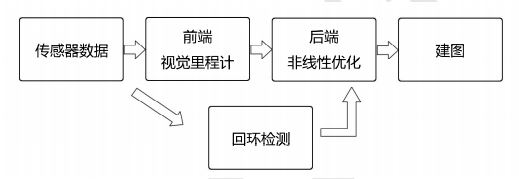
\includegraphics [scale=0.45,trim=0 0 0 0]{./image/SLAM_workflow}
	\bicaption[fig_id1_workflow]{图}{\centering 视觉SLAM工作流程图}{Fig.}{\centering Workflow of Visual SLAM}
\end{figure}

以上是经典的视觉SLAM工作流程框架,其在过去的几十年间已有较为丰硕的研究成果,这个框架所包含的研究成果基本定型。在现有的开源机器人程序库中,完全可以依靠这些现有算法搭建一个SLAM系统。由于本文主要研究视觉里程计,所以,以下对视觉里程计进行详细的介绍。

视觉里程计关心的是相邻图像间的相机的运动,也即是如何通过相邻的两幅图像估计相机的位姿变换情况。在现实世界中,人眼能够很轻易地通过视觉中镜像的变换感受出自己身体的运动在状态\cite{maer},在图\ref{fig_id2_eye}中,我们人眼能够很轻易的通过图像从左到右的变化猜测出人眼向左旋转或者移动了,因为左边的景物明显变多了。但是如果进一步深究,人眼移动了多少,这样一个量化的问题是难以回答的,因为我们的直觉对数字并不敏感。所以,计算机相比我们,其优势就是可量化地表示出这种量化。在计算机视觉中,图像的表示方式是一个数值矩阵,如何通过一系列的数值矩阵估计相机的运动,就是视觉里程计的本质工作。但是,如果仅仅通过视觉里程计来估计相机的运动轨迹,难免会出现漂移,因为视觉里程计是独立地估计两幅间的运动,每次估计只与上一幅图像相关,所以就会出现误差累计的现象。这导致经过一段时间后,估计的轨迹不再准确。解决这个问题就是后端检测的任务,在此不细讲。

\begin{figure}[h!]
	\centering
	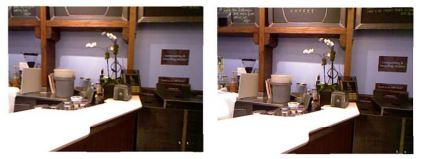
\includegraphics [scale=0.5,trim=0 0 0 0]{./image/eyes_image}
	\bicaption[fig_id2_eye]{图}{\centering 运动产生的图片变化}{Fig.}{\centering Workflow of Visual SLAM}
\end{figure}

\section{在SLAM问题中为什么需要视觉里程计}
\enlargethispage{-3.3cm}
理解这个问题需要对SLAM过程进行数学语言的描述。根据文献\cite{dummies}介绍,假设环境有许多\textbf{路标}(landmark)组成,将机器人连续运动变成离散的时刻:t=1、2......K。图\ref{fig_id3_landmark}为机器人在某一时刻的运动及工作状态,其中五角星表示路标,虚线的三角形表示里程计估计的机器人的位置(称为位置1),淡实线表示机器人根据对landmark的观测确定的机器人位置(称为位置2),深实线表示机器人实际所在的位置(称为位置3)。假设机器人携带一个测量自身运动信息的传感器,通过这个传感器可以测量自身运动的里程信息,这个传感器可以是码盘,IMU或者相机(此时则是视觉里程计),但无论这个传感器是什么,我们都可以将机器人的运动状态表示如下:

\begin{equation}s
\label{sport}
x_{k} = S(x_{k-1},u_{k},w_{k})
\end{equation}

这里 $u_{k}$ 是k时刻传感器的读数,$w_{k}$是k时刻的噪声,$u_{k-1}$是上一时刻机器人所在的位置,$u_{k}$是机器人当前所在位置。机器人运动的原点为机器人开机后机器人所在的位置。式\ref{sport}也称为机器人的运动方程。与运动方程相对的,称为观测方程:

\begin{equation}
\label{observe}
z_{k,j}=O(y_{j},x_{k},v_{k,j})
\end{equation}

式中$ y_{j} $为机器人在$ x_{k} $位置观测到的路标,$ z_{k,j} $ 为k时刻,根据该路标产生的观测数据,$ v_{k,j} $代表噪声。因为该方程是根据外界观测信息对机器人自身的信息(比如位置信息)进行估计,所以式\ref{observe}称为观测方程。

\begin{figure}[h!]
	\centering
	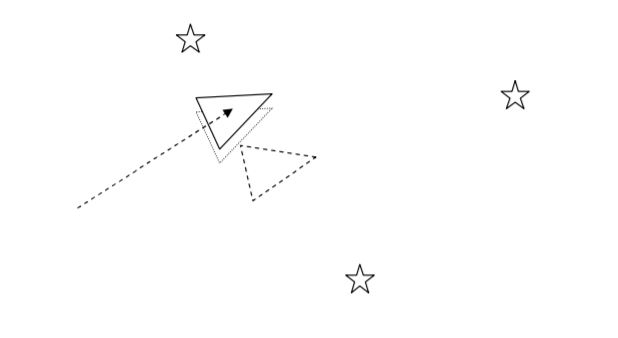
\includegraphics [scale=0.4,trim=0 0 0 0]{./image/landmark}
	\bicaption[fig_id3_landmark]{图}{\centering 机器人自我定位原理}{Fig.}{\centering Workflow of Visual SLAM}
\end{figure}

结合式\ref{sport} \ref{observe}以及图\ref{fig_id3_landmark},机器人根据运动方程计算出机器人在k时刻处于位置1,然后又根据观测方程观测自己位于位置二。可以看出,运动方程对机器人自身位置的估计准确度比观测方程低。但是这是不是意味这里程计信息是多余的呢?将上面的分析过程进一步拓展,令$ x_{k} = [x,y,\theta]_{k}^{T} $,即机器人的位姿。$ u_{k} = [\delta x ,\delta y, \delta \theta] $,代入式\ref{sport}

\begin{equation}
\left[ \begin{array}{ccc}
x\\
y\\
\theta
\end{array} 
\right ]_{k} = \left[ \begin{array}{ccc}
x\\
y\\
\theta
\end{array} 
\right ]_{k-1} + \left[ \begin{array}{ccc}
\delta x\\
\delta y\\
\delta \theta
\end{array} 
\right ]_{k} + w_{k}
\end{equation}

对于观测方程,我们假设路标$ y_{j} = [p_{x},p_{y}]^{T} $,观测数据$ z_{k,j} = [r,\theta]^{T} $,其中r为机器人相对路标的距离和夹角。可将观测方程写成:

\begin{equation}
\left[ \begin{array}{ccc}
r\\
\theta
\end{array} 
\right ] = \left[ \begin{array}{ccc}
\sqrt{(p_{x}-x)^2 + (p_{y}-y)^2}\\
\arctan \dfrac{p_{y}-y}{p_{x}-x}
\end{array} 
\right ] + v
\end{equation}

以上两个方程描述了SLAM的基本过程,由于使用的传感器不同,具体方程的具体形式根据实际的情况变化而变化,。根据以上两个方程可以解决SLAM的基本问题:定位与建图,事实上,定位问题指的就是估计机器人位姿x的问题,建图问题则是对路标y进行估计的问题。这样,SLAM问题其实就是对x,y的在噪声中的状态估计问题。而状态估计问题的求解,根据噪声是否服从高斯分布、运动和观测方程是否线性,分为高斯/非高斯和线性/非线性系统\cite{robust},所以有如下四种SLAM系统:

\begin{table}[h]
	\centering
	\captionnamefont{\xiaowuhao\bf }
	\captiontitlefont{\xiaowuhao\bf }
	\bicaption[labelTabtab1]{表}{SLAM系统类型}{Table}{Type of SLAM}
	\renewcommand\tabcolsep{1em}
	% \xiaowuhao \selectfont
	% \renewcommand{\arraystretch}{0.8}
	% \fontsize{9}{11}\selectfont
	\begin{tabular}{cc}
		\toprule
		{编号} &  {类型}\\
		\midrule 
		1 & 线性高斯 \\
		2 & 非线性非高斯\\
		\bottomrule
	\end{tabular}
\end{table}

线性高斯系统式最简单的系统,其最优估计可由卡尔曼滤波(Kalman Filter,KF)给出,而非线性非高斯系统则是最复杂的系统,其代表的求解方法有拓展卡尔曼滤波(Extend Kalman Filter,EKF)和非线性优化\cite{gaoxiang14slam}。由于现实环境基本多是非线性非高斯,于机器人鲁棒性而言,将SLAM系统设计成非线性非高斯的,明显是更优的。事实上,最早的实时视觉SLAM系统则是基于EKF开发的,但是由于EKF假设噪声分布是高斯分布,误差是线性化的,所以EKF还不那么符合现实环境的特点。而后人们开始使用粒子滤波器,随着计算机能力以及非线性优化技术的提高,当前主流的SLAM基本偏向于使用非线性优化技术。

至此,还未回答本节的目标问题:为什么SLAM系统需要视觉里程计?似乎根本不需要运动方程,我们就可以根据观测方程得到机器人的位置。事实上,由于SLAM问题是一个状态估计问题,所以机器人其实只是“猜测”自己实际所在的位置以及路标的位置,机器人
 
\section{正文}
\subsection{量、单位、公式}
\subsubsection{公式编排}
\label{labSecForm}
《北京航空航天大学学报》一般不编排单独的符号表,对于公式中的变量含义需要说明的,请在公式后的段落中,采用``式中:$A$为某某;$B$为某某;……"的方式加以说明。
\begin{equation}
\label{eqnLabelp}
p_1 (h) = \dfrac{n_{\textnormal{He}}RT}{V}-\rho_{\textnormal{He}}gh
\end{equation}
式中:$n_{\textnormal{He}}$ 和 $\rho_{\textnormal{He}}$ 分别为艇囊内部氦气的物质的量和氦气在温度 $T$ 时的平均密度;
$V$=\SI{36893.426}{\cubic\meter}%%数字会小一些,默认的是公式字体大小
为艇囊体积;$T$=\SI{216.65}{\kelvin}为艇囊内稳态温度;$h$为距离艇囊中心轴线($x$轴)的垂直高度.请使用Mathtype编辑。公式中字体的定义尺寸为10磅,上标/下标68\%,次下标/上标42\%,符号150\%,次符号100\%(设置方法:Mathtype-尺寸-定义)。长公式如需转行,应在记号=,+,$-$等之后断开,而在下一行开头不再重复这一记号。

\subsubsection{量和单位}
有关记号的使用应符合国家标准,例如:$\sin^{-1}$应为$\arcsin$,$\rm ctg$应为$\cot$,$\rm tg$应为$\tan$,不要使用非国家法定单位,如ppm等表示法已要求停止使用(rpm应写为r/min);除$Re$, $Ma$(其中$e$, $a$不是下标)等几个特征数外,变量应使用单个字母表示,可以带上标和下标(否则由多个字母表示单个变量,易被误解为多个变量相乘)。

\subsubsection{字体}
矩阵、向量请用粗斜体表示,变量用一般斜体表示;下标字母若为说明性的(如英文缩写)则用正体表示,若为量和变动性数字及坐标轴的符号则用一般斜体表示(设置方法:Mathtype-样式-定义-高级)。

所有文中出现的符号请另附文档说明其是变量、向量等,并说明各变量上下标的含义,以便编辑确定它们应采用的排版字体(变量符号说明表)。

请作者对易于混淆的字母和数字,如数字0和字母o,英文a和希腊字母$\alpha$,O,P,S,C等的大小写,批注``英大"(代表英文大写)、``数字0"、``希小"(代表希腊字母小写)等。

\subsection{图、表}
图、表需给出中英文图题、表题(子图也需给出图题),但图表中图例、线型说明等一律用中文。图表一般不超过7.7\ cm宽。金相图和计算机云图,其中的比例尺等字编辑过程中都不再重贴,按照照片处理,如有这两类图请保证美观清晰,字体用times new roman。

\subsubsection{图片}
对于函数曲线图,采用全框图,并注意检查以下各项:

1)横纵坐标的标目(即变量名),尽量使用国标变量符号,变量名要在正文中交待,且与正文中符号一致;若正文中无,也可使用中文名称。

2)坐标轴标目的量纲,对于无量纲化或无单位的,请注明``无单位”。

3)坐标轴上的刻度线朝内,刻度值完整(坐标轴始末点均应有完整刻度值)。

4)不同线型或图符是否有说明。

5)是否矢量图格式,从软件中输出或拷贝矢量图格式直接插入文档中,避免用拷屏办法插图图片,否则后期无法编辑。

6)类似图片尺寸尽量相同。

《北航学报》自2014年起可提供彩版印刷,如有彩印需求请作者在“出版工作单”中注明。若不需彩印,请作者作图时注意用可区分的线形或符号区分不同曲线,以保证黑白图清晰可分辨。 

图中文字均用中文或变量名称表示!
\begin{figure}[b!]
\centering
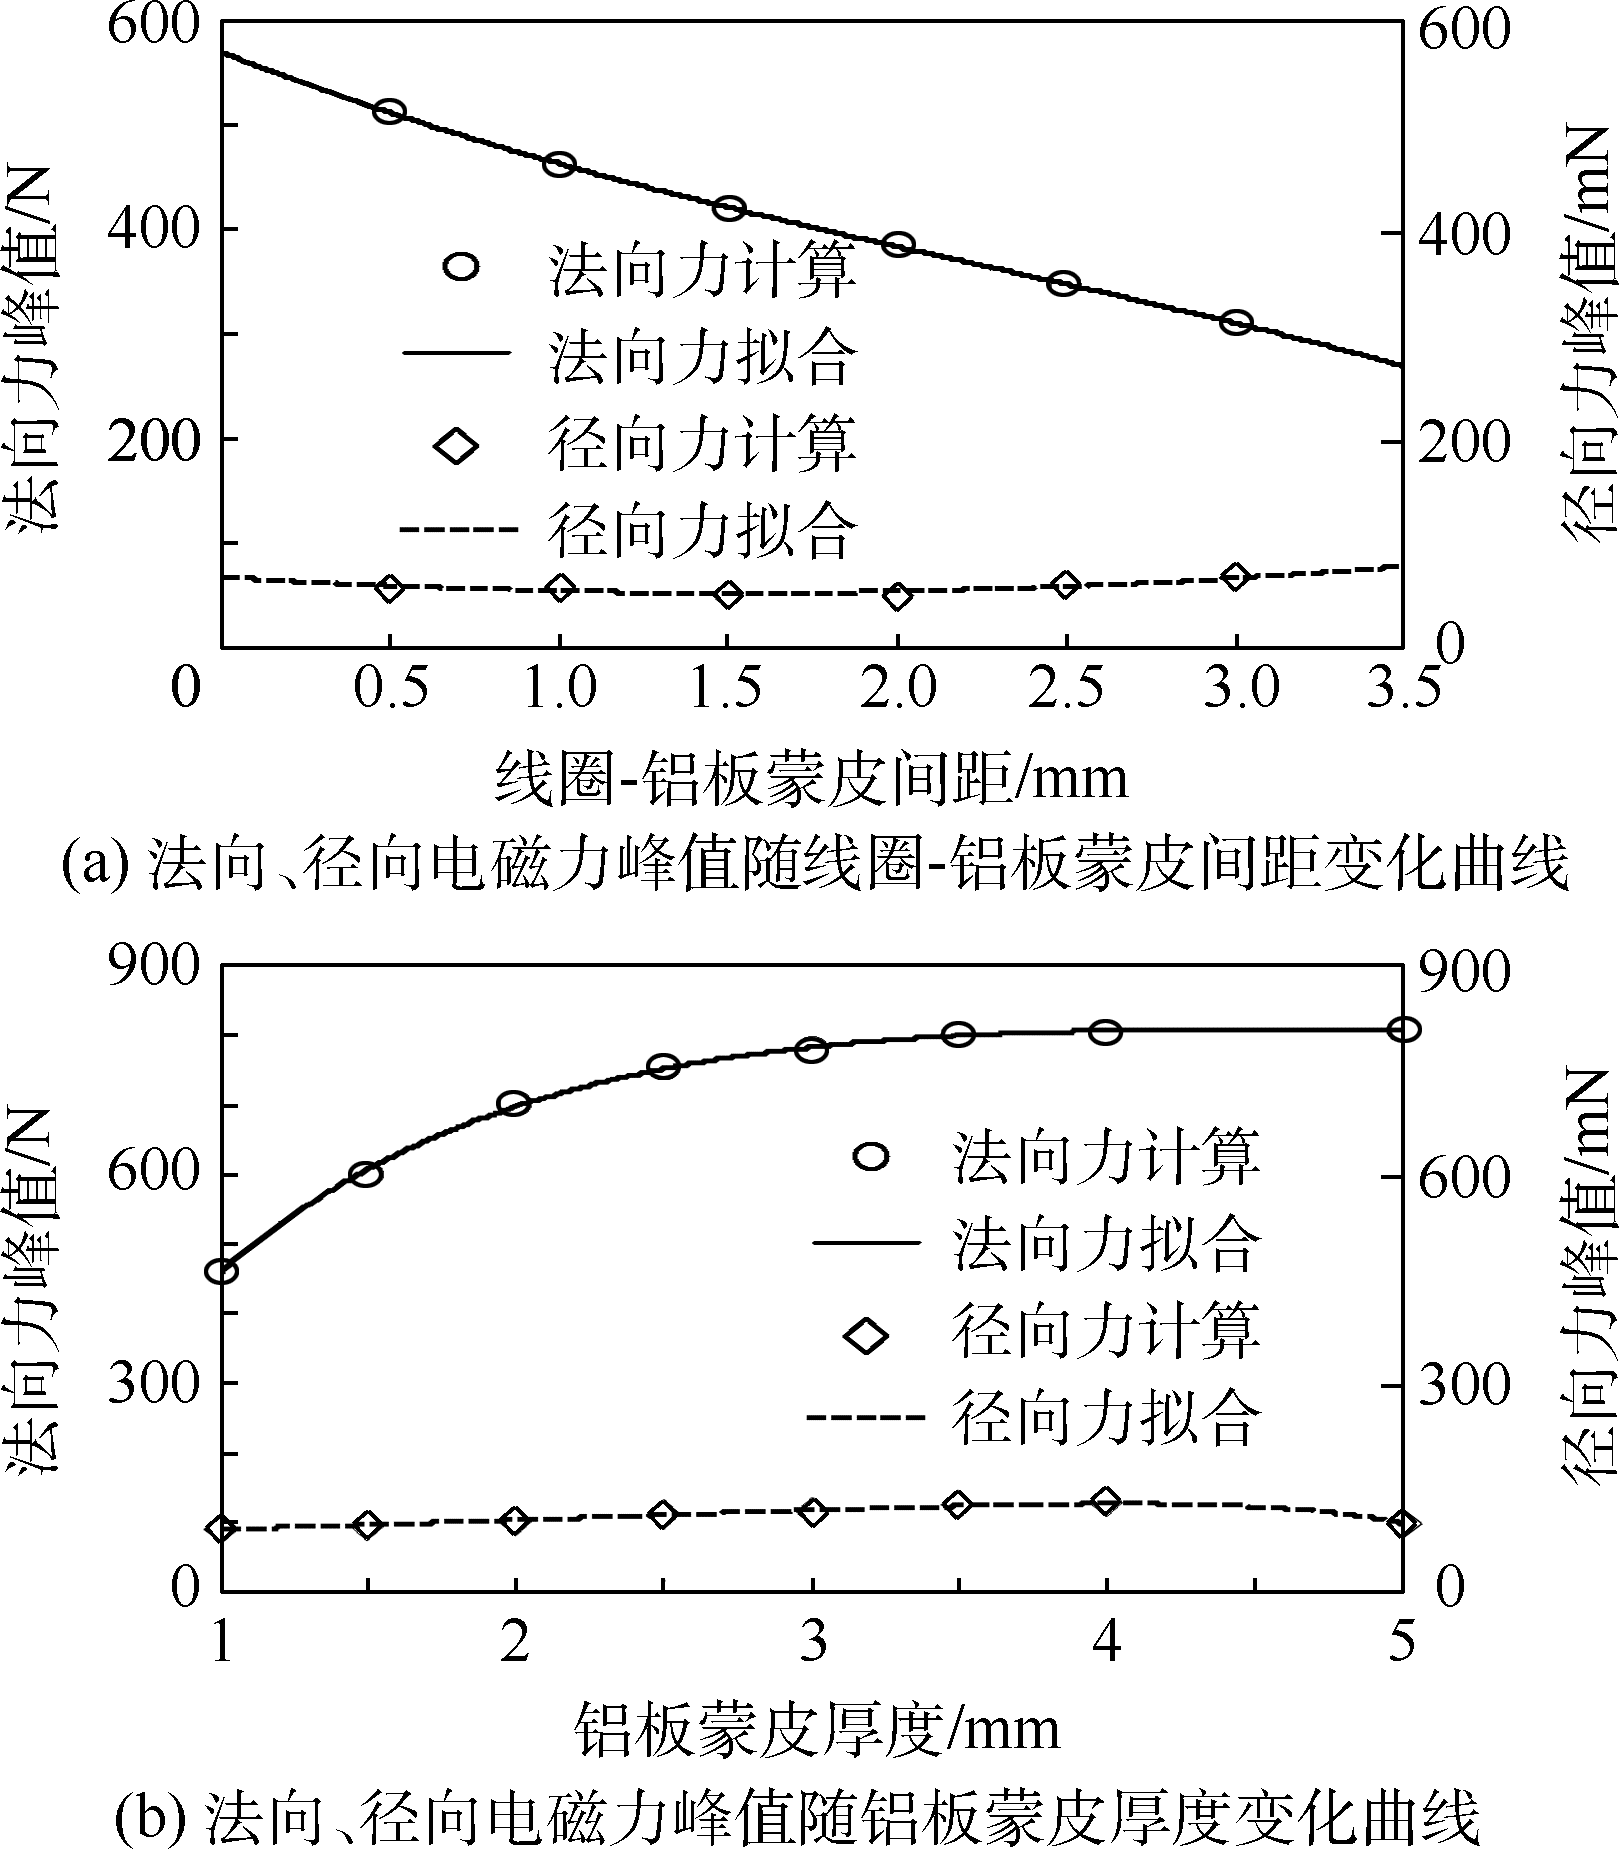
\includegraphics [scale=1,trim=0 0 0 0]{./image/tu1.png}
\bicaption[labelFigtu1]{图}{\centering 电磁力峰值随线圈-铝板蒙皮间距和铝板蒙皮厚度变化曲线}{Fig.}{\centering Curves of electromagnetic force peak changing with coil-aluminum-plate gap and thickness of aluminum plate}
\end{figure}

图片样例见图\ref{labelFigtu1}和图\ref{labelFigtu2}(目前是位图格式,不能编辑,作者应提供可编辑的矢量图)。

\begin{figure}[h!]
\centering
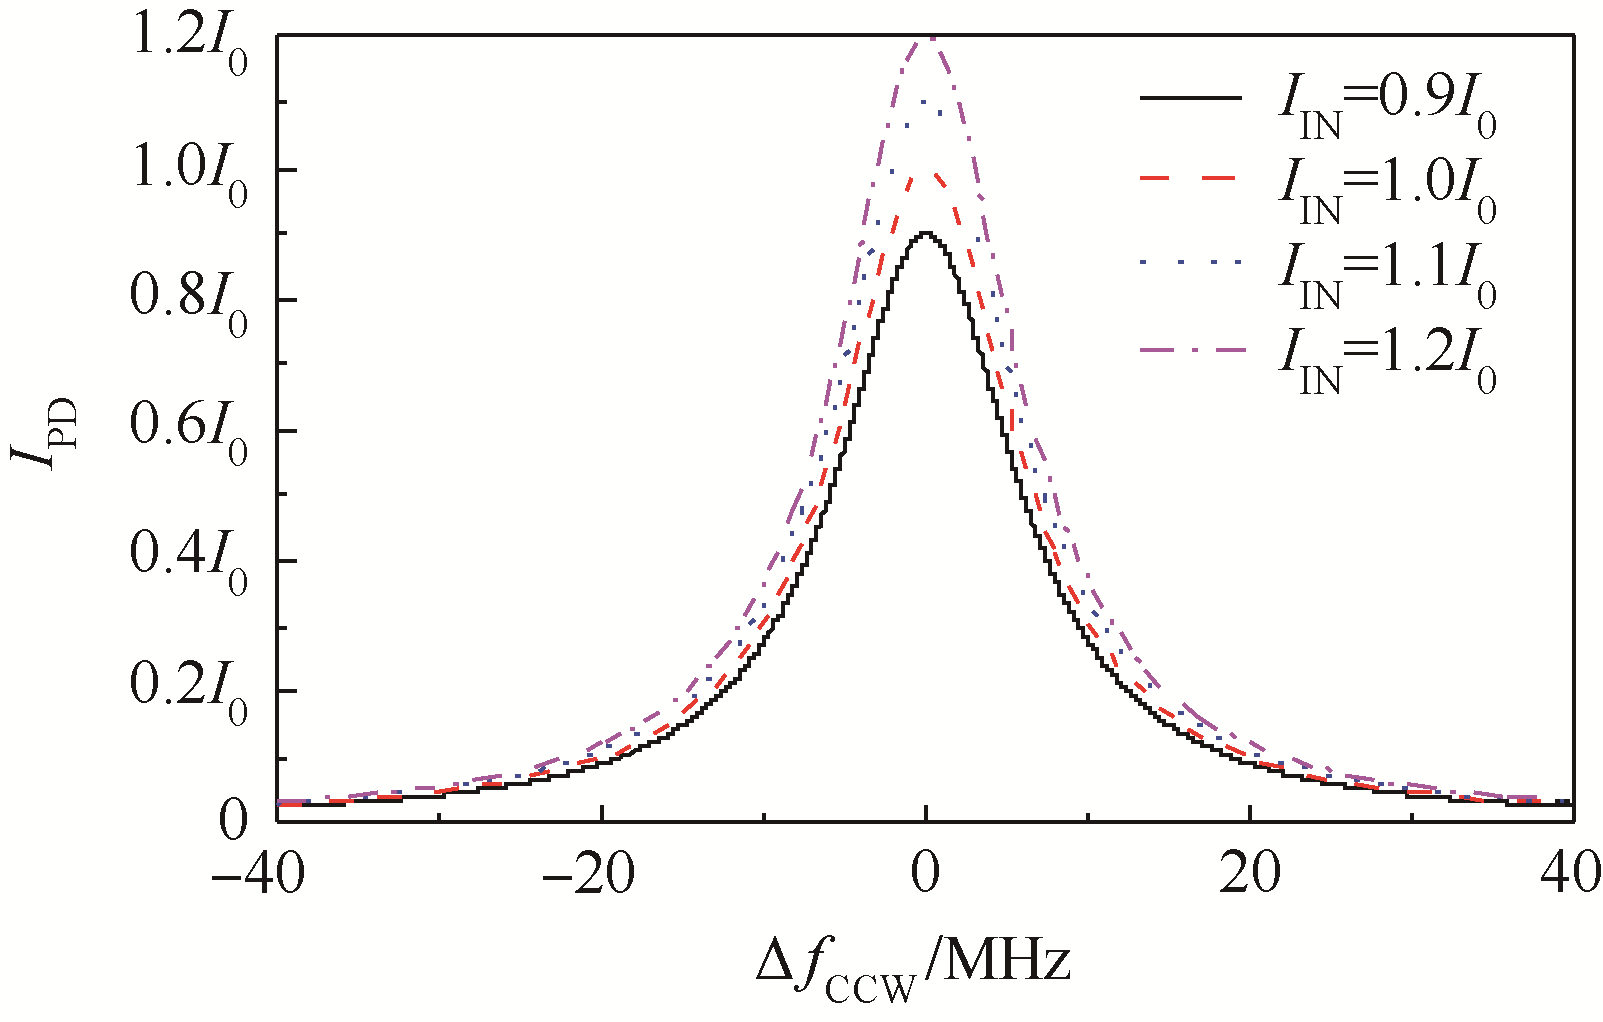
\includegraphics [scale=1,trim=0 0 0 0]{./image/tu2.png}
\bicaption[labelFigtu2]{图}{\centering 谐振腔输入光强波动对谐振曲线的影响}{Fig.}{\centering Fluctuation influence of the resonator's input intensity on resonance curve}
\end{figure}

\subsubsection{表格}
请使用三线表。选中表格,点右键打开``边框和底纹”,可对表格的边框等格式进行编辑,三线表的一般格式见表\ref{labelTabtab1}。
\begin{table}[h]
\centering
\captionnamefont{\xiaowuhao\bf }
\captiontitlefont{\xiaowuhao\bf }
\bicaption[labelTabtab1]{表}{传输线积冰条件}{Table}{Icing conditions of transmission line}
\renewcommand\tabcolsep{1em}
% \xiaowuhao \selectfont
% \renewcommand{\arraystretch}{0.8}
% \fontsize{9}{11}\selectfont
\begin{tabular}{cccc}
\toprule
{编号} &  {直径}/\si{\metre} & {静温}/\si{\kelvin} & {时间}/min\\
\midrule 
4 & 0.0349 & 268.15 & 30\\
5 & 0.01905 & 268.15 & 30\\
\bottomrule
\end{tabular}
\end{table}

\subsubsection{计算、实验}
文章以数值计算为主要内容的,应给出所求解的方程、重要的计算参数、初始或边界条件、难点问题的处理等,应对方法的适用性和计算精度估计有所说明;文章以实验为主要内容的,应说明实验设备、实验条件,对实验误差的估计等。便于同行重复再现所报道的内容,由于保密原因不便公开某些内容的,应向责任编辑说明。

\section{参考文献}
1) 引用文献应遵循``最新、关键、必要和亲自阅读过”的原则;

2) 参考文献应是公开出版物;

3) 应在正文中顺次引述(按在正文中被提及的先后来排列各篇参考文献的序号,所有参考文献均应在正文中提及);

4) 文献条数15条以上,且有适量近两年文献;

5) 参考文献中作者为3人或少于3人应全部列出,3人以上只列出前3人,后加``等”或``et al”;

6) 参考文献中外国人名书写时一律姓前,名后,姓用全称大写,名缩写为首字母(大写),不加缩写点;

7) 为便于国际交流,对外文文献按外文著录;对于中文文献首先按中文著录,同时提供英文对照,并在其后注 ``(in Chinese)” 注意对中文期刊刊名应使用其标准译法(通常在文章首页页眉可以找到)。

具体样例详见文后参考文献部分。

\begin{table}[h!]
\centering
\captionnamefont{\xiaowuhao\bf }
\captiontitlefont{\xiaowuhao\bf }
\bicaption[labelTabtab2]{表}{文献类型和标志代码}{Table}{Referrence type and identification code}
\liuhao
\tabulinesep=1.2mm
\begin{tabu} to 0.95\linewidth {X[c,m] X[1,c,m]|[1pt]X[1,c,m] X[1,c,m]}
\tabucline[1pt]{-}
{参考文献} &  {文献类型} & {参考文献} &  {文献类型} \\
{类型} &  {标识} & {类型} &  {标识}\\ \hline
    专著     &  M  & 学位论文  & D     \\
    会议录    &  C  &  报告   &   R   \\
    期刊     &  J  & 标准    &   S   \\
    报纸     &  N  & 专利    &   P   \\
    汇编     &  G  & 档案    &   A   \\
    计算机程序 & CP  &电子公告  &   EB    \\
    数据库    & DB &美图      &  CM   \\
    数据集    & DS &其他      &    Z  \\ \tabucline[1pt]{-}
\end{tabu}
\end{table}

 \begin{table}[h!]
\centering
\captionnamefont{\xiaowuhao\bf }
\captiontitlefont{\xiaowuhao\bf }
\bicaption[labelTabtab3]{表}{电子文献载体和标志代码}{Table}{Electronic literature and identification code}
%\renewcommand\tabcolsep{2pt}
\liuhao
\tabulinesep=1.2mm
\begin{tabu} to 0.98\linewidth {X[c,m] X[1,c,m] X[1,c,m] X[1.35,c,m] X[1.2,c,m]}
\tabucline[1pt]{-}
\makecell{载体\\ 类型} &  \makecell{磁带\\ (magnetic\\ tape)} & \makecell{磁盘\\ (disk)} & \makecell{光盘\\ (CD-ROM)} & \makecell{联机网络\\ (online)}\\
\hline
\makecell{标志\\ 代码} & MT & DK & CD & OL\\
\tabucline[1pt]{-}
\end{tabu}
\end{table}

\section{其他有关事项说明}
1) 文章应着重撰写创新性、关键性内容,并以一般专业人员看得懂为原则

2) 返回时间:修改稿一般应在10天内返回,或以责任编辑的要求为准。如作者不能按时返回,请向责任编辑说明情况

3) 返回文件(请从系统上传):

\circled{\xiaowuhao 1} 论文电子版(修改部分用不同颜色标识)

\circled{\xiaowuhao 2} 论文修改说明(写明对专家及编辑部所提意见如何修改)

\circled{\xiaowuhao 3} 变量符号说明表(模板见下载园地)

\circled{\xiaowuhao 4} 稿件出版工作单(word版,模板见下载园地);``稿件出版工作单"中有关事项请认真填写,联系电话最好有手机。后期编辑及发行过程中,会根据作者填写的信息与作者联系解决稿件问题,联系方式及寄刊地址有变更的,请及时通知责任编辑

稿件修改期间请对修改稿仔细审读、精加工,一经排版,一般不允许做大的改动

4) 出版过程:责任编辑在编辑修改稿过程中常会有疑问请作者答复补正,请作者配合及时答复;稿件修改符合要求后,责任编辑将根据文章页码经电子信箱发送缴纳版面费通知单,作者应根据通知单要求及时缴纳版面费;编辑部有权对文章进行文字性修改,使之符合出版体例、规范要求和篇幅限制;责任编辑在编完稿件后,将其转至总编辑处,按来稿先后顺次发表;文章出版后,免费向作者提供样刊和抽印本,每篇文章1本样刊及5本抽印本,如作者需要可另购样刊,刊款可随版面费一并缴纳

5) 提前发表:本刊一般发表周期为1年,作者若有特殊情况确实需要提前发表的,请提前向学术编辑联系及说明情况,编辑部可根据实际情况适当安排

\section{结~~论}
分点总结,列出具体结论,其他背景、方法都不必赘述。不与摘要和前言重复。具体样例如下:

1) 算法可实现较为优异的检索性能,例如返回10张结果条件下算法检索正确率83.15\%,召回率8.42\%,在60张下正确率39.33\%,召回率24.61\%。

2) 算法提出单张图片的引入不会造成原图片库的特征向量集和主题概率分配发生严重畸变的两个假设在一定范围(待检索图片与原图库特征类似)内是成立的。

3) 算法的预备工作使检索范围由原先整个库缩小至某个子类中,虽使召回率有所损失,但检索时间得到较大的缩短。

4) 可预估对于特征较接近的图片库,比如人脸库,图片预备工作会产生较大的分类误差,且可能进一步影响检索性能。

为使本文提出的算法能处理各种类型的图片,仍需要优化预备工作和检索实现过程的各项参数。


\section{\mycolorRed{模板中一些问题}}

1) 所有\mycolorRed{间距}都是手动设置,可能与word模板有些差别。包括正文行间距、各级节标题前后行间距、文本字与字间距、页面设置(页边距)、双栏间距、公式前后间距、图表(标题)前后间距、页眉页脚间距等等

2) \mycolorRed{字体}设置;正文中文、英文均是五号字(10.5pt),而公式中设置为10pt,所以公式中数字会小于普通文本数字,如$x=5$和5;带单位的量采用siunitx生成的话也有这个问题,如速度为\SI{5}{m/s}和5\ m/s。公式中上下标看起来与word版稍有差别;公式中$g$与word版\textit{g}也不同,默认公式字体可能并不是times new roman,本模板里未设置。

3) \mycolorRed{双栏}设置,采用的是article模板twocolumn选项;multicol对浮动图表支持要差一些;twocolumn也有些问题,比如首页跨两栏的脚注,没找到更好的办法,这里使用了\textbackslash enlargethispage\{\}预留出脚注位置,然后用tikz手动调node的位置。还有跨两栏的图表灵活性稍差,\{figure*\}。

4) 图表中英文题注,使用ccaption得到。公式中向量矩阵粗斜体可以使用\textbackslash bm得到。

5) 参考文献,为了自动排序,引用方便,使用BibTex,但是参考文献格式不属于标准的,所以所有参考文献只使用misc这个entry,而且只用到misc中note这一个field,也就是把整条参考文献都放到note里了。工作量与word差不多,但是引用、增删排序更方便些。

6) 变量符号说明表,里面加了一列符号所在位置,需要用到本文件生成的辅助文件,里面有可以引用的label信息。


\vspace{1em}
{\hei\wuhao 致谢\quad}
{\fang\wuhao 
感谢某某……注意:首页注明基金项目后,文末不必再致谢。
}



%%%%%%%%%%%%%%%%%%%%%%%%%%%%%%%%%%%%%%%%%%%%%%%%%%%%%%%%%%%%%%%%
%  参考文献
%%%%%%%%%%%%%%%%%%%%%%%%%%%%%%%%%%%%%%%%%%%%%%%%%%%%%%%%%%%%%%%%

\renewcommand\refname{\hei\wuhao\centerline{参考文献(References)}\global\def\refname{参考文献}}
\vskip 12pt

\let\OLDthebibliography\thebibliography
\renewcommand\thebibliography[1]{
  \OLDthebibliography{#1}
  \setlength{\parskip}{0pt}
  \setlength{\itemsep}{0pt plus 0.3ex}
}

{
\renewcommand{\baselinestretch}{0.9}
\liuhao
\bibliographystyle{unsrt}
\bibliography{./TempExample}
}



%%%%%%%%%%%%%%%%%%%%%%%%%%%%%%%%%%%%%%%%%%%%%%%%%%%%%%%%%%%%%%%%
% 作者简历
%%%%%%%%%%%%%%%%%%%%%%%%%%%%%%%%%%%%%%%%%%%%%%%%%%%%%%%%%%%%%%%%
{
\xiaowuhao
\noindent {\hei 作者简介:}

\noindent {\hei 姓名}~~~ 性别,学历,职称。主要研究方向:xxxxxxxxxx。
\vskip 16pt

\noindent {\hei 张某某}~~~ 男,博士研究生。主要研究方向:xxxxxxxxxx。
\vskip 16pt

\noindent {\hei 李某某}~~~ 男,博士,教授,博士生导师。主要研究方向:xxxxxxxxxx。
}

%%%%%!!!!!需要在合适位置插入\newpage,来平衡最后一页两栏!!!!!
% \newpage  %%% 用于平衡最后一页两栏高度

%%%%%%%%%%%%%%%%%%%%%%%%%%%%%%%%%%%%%%%%%%%%%%%%%%%%%%%%%%%%%%%
% % % 附录
%%%%%%%%%%%%%%%%%%%%%%%%%%%%%%%%%%%%%%%%%%%%%%%%%%%%%%%%%%%%%%%
\vskip 20pt
 
 \noindent {\hei 附录A:}
 
若确有特殊需要设附录的,附录部分置于作
者简介后,标题为“附录A:”、“附录B:”......。公式
用大写字母和数字顺序编号,例如“(A1)”, “(A2)”。




%%%%%%%%%%%%%%%%%%%%%%%%%%%%%%%%%%%%%%%%%%%%%%%%%%%%%%%%%%%%%%%%
%  英文摘要页
%%%%%%%%%%%%%%%%%%%%%%%%%%%%%%%%%%%%%%%%%%%%%%%%%%%%%%%%%%%%%%%%
\clearpage
\newpage
% \cleardoublepage
% \cleardoublepage\null
% \newpage\null\thispagestyle{empty}\newpage
\pagestyle{fancy}
\fancyhf{}
\lhead{}
\chead{\vspace{0.8cm}\centering{{\CJKfamily{hei}\xiaowuhao 特别鸣谢tex如此好用的写作工具}\\[-0.5ex]
{{\xiaowuhao}}}}
\rhead{}
\lfoot{}
\cfoot{}
\rfoot{}
\renewcommand{\headrule}{%
\hrule height0.4pt width \headwidth \vskip1.0pt%
\hrule height0.4pt width \headwidth \vskip-2pt}
%%%%%%%%%%%%%%%%%%%%%%%%%%%%%%%%%%%%%%%%%%%%%%%%%%%%%%%%%%%%%%%%
%          英文摘要
%%%%%%%%%%%%%%%%%%%%%%%%%%%%%%%%%%%%%%%%%%%%%%%%%%%%%%%%%%%%%%%%

\twocolumn[
  \begin{@twocolumnfalse}\vspace*{0.3cm}
\begin{center}
\parbox{\textwidth}{
\setlength{\parindent}{1em}
{
\centering\sihao\textbf{Title title title title title title} \xiaowuhao\fang (不超过10个实词,不出现非公知公用的缩写词)\\
} \vspace{-1.2mm}
\begin{center}
{\wuhao ZHANG Moumou\makebox{$^{\text{1,2}}$}, LI Mou\makebox{$^{\text{1,2,*}}$}, SHANGGUAN Moumou\makebox{$^{\text{2,3}}$}, LIN Mou\makebox{$^{\text{3}}$}, ZHAO Mou\makebox{$^{\text{3}}$}, WANG Mou\makebox{$^{\text{3}}$}}\\[-0.1cm]
\liuhao{(1. School of Aeronautic Science and Engineering, Beijing University of Aeronautics and Astronautics, Beijing 100191, China;\\
2. School of Astronautics, Beijing University of Aeronautics and Astronautics, Beijing 100191, China;\\
3. College of Automation, Northwestern Polytechnical University, Xi’an 710072, China)}
\end{center}

\vspace{-10pt}\wuhao
{
\textbf{Abstract:} 
(与中文摘要内容对应,英文摘要字数150\textasciitilde 200个单词)英文摘要应和中文摘要对应,并请导师
或专业人士把关,保证摘要质量,高质量的摘要有利于文摘被国际权威数据库收录,及引起同行的重视。
如果英文摘要比中文摘要更详细,应另提供一份英文摘要的中文副本,以便于本刊英文编辑检查英文。
首次出现英文缩写时应注意写明全称。

英文摘要的撰写规范请参考本刊网站“下载园地”中的《Ei文摘要求》。

\textbf{Key words:} keyword1; keyword2; keyword3; keyword4; keyword5(与中文关键词一一对应,关键词请尽量从EI Controlled term中选择,以提高 EI检索的命中率及被引频次,网址:http://www.engineeringvillage.com/search/quick.url)。
}
}
\end{center}

%%%%%!!!!!英文脚注!!!!!
\positiontextbox{2.0cm}{16cm}{
\noindent\rule{4cm}{.5pt}\\[0.5ex]%
\hspace*{1em} \xiaowuhao \linespread{0.8}\selectfont
\parbox{\textwidth}{%
\CalibriFont
\hei\makebox[\widthof{\makebox{*}\textbf{R}}][r]{\textbf{R}}\textbf{eceived:} 2017-xx-xx; \textbf{Accepted:} 2017-xx-xx; \textbf{Published online:} 2017-xx-xx xx:xx\\%
\hei\makebox[\widthof{\makebox{*}\textbf{U}}][r]{\textbf{U}}\textbf{RL:} \\
\hei\makebox[\widthof{\makebox{*}\textbf{F}}][r]{\textbf{F}}\textbf{oundation item:} National Natural Science Foundation of China (12345678); China Postdoctoral Science Foundation(87654321)\\ 
\hspace*{2em}(注:基金项目英文名称查询“基金项目的中英文名称”) \\
\hei\makebox[\widthof{\makebox{*}\textbf{C}}][r]{\makebox{*}\textbf{C}}\textbf{orresponding author.} Tel.: 010-8231xxxx ~~ E-mail: bhxb@buaa.edu.cn
}}
  \end{@twocolumnfalse}
]

%%%%%%%%%%%%%%%%%%%%%%%%%%%%%%%%%%%%%%%%%%%%%%%%%%%%%%%%%%%%%%%%
%  英文摘要页 结束
%%%%%%%%%%%%%%%%%%%%%%%%%%%%%%%%%%%%%%%%%%%%%%%%%%%%%%%%%%%%%%%%

\end{document}
